\documentclass{beamer}
\usetheme{Madrid}

\AtBeginSection[]{
	\begin{frame}
	\vfill
	\centering
	\begin{beamercolorbox}[sep=8pt,center,shadow=true,rounded=true]{title}
		\usebeamerfont{title}\insertsectionhead\par%
	\end{beamercolorbox}
	\vfill
	\end{frame}
}

\newcommand{\pic}[1]{
\begin{figure}
\vspace{1cm}
\includegraphics[width=0.3\textwidth]{img/#1}
\end{figure}
}


\title{CokieGraph:
Understanding and Detecting First-Party Tracking Cookies}

\author{Robert Krzysztof Noparlik}


\begin{document}

\begin{frame}
\titlepage
\end{frame}

\begin{frame}
\frametitle{Outline}
\tableofcontents
\end{frame}


\section{What is this about?}


\begin{frame}
\frametitle{Problem}
\begin{itemize}
\item 3rd party cookies are increasingly being blocked in browsers
\item Advertisers now use 1st party cookies to track users. 

\pic{cookie}

\end{itemize}
\end{frame}


\begin{frame}
\frametitle{Contribution}

\begin{itemize}
\item CookieGraph - block the offending first party cookies in order to stop tracking.
\item Measure how 3rd party cookies actually stop the tracking.
\end{itemize}
\end{frame}

\begin{frame}
\frametitle{Result}

\begin{itemize}
\item Over 90\% of first party tracking cookies blocked by CookieGraph - the best of any other solutions.
\item Large overhead - infeasible to run in an \textit{offline} mode on consumer hardware.
\item Most tracking happens with first-party cookies anyway.
\end{itemize}
\end{frame}

\begin{frame}
\frametitle{Meaning}
\begin{itemize}
\item Blocking third party cookies barely makes a difference in the amount of tracking.
\item However, it's possible to detect and block first-party cookies. But, it requires a lot of computing power.
\end{itemize}
\end{frame}


\section{Motive}

\begin{frame}
\frametitle{3rd Party Cookie Blocking}

\pic{ie}

\begin{itemize}
\item Most browsers adopting countermeasures against tracking through 3rd Party Cookies.
\item A new way of tracking is needed for advertisers.
\end{itemize}

\end{frame}

\begin{frame}
\frametitle{Use 1st Party Cookies?}

\begin{itemize}
\item Set an ID.
\item Exfiltrate this ID in connection with other \textit{PPID} like emails or a browser fingerprint.
\item Connect user through different sites and devices.
\end{itemize}

\end{frame}

\begin{frame}
\frametitle{How can we protect against this tracking?}

\begin{itemize}
\item Existing solutions don't work as well and are based on things like domain names.
\item Blocking requests sometimes causes websites to become unusable (eg. AdBlock).
\end{itemize}

\end{frame}

\begin{frame}
\centering
A need for a dedicated solution.

\pic{solution}
\end{frame}


\section{Backround}

\begin{frame}
\frametitle{1st vs 3rd party cookies}
\begin{itemize}
\item Cookies can be set either by \textit{Set-Cookie} response header or \textit{document.cookie}.
\item When \textit{Set-Cookie} is used in a response from the \textit{same} domain as the site, it's a 1st party cookie.
\item When \textit{document.cookie} not in third party context (not in iframe), it's a 1st party cookie.
\end{itemize}
\end{frame}

\begin{frame}
\centering
What about 1st party cookies?
\end{frame}


\begin{frame}
\frametitle{1st Party Cookies for tracking}

\begin{itemize}
\item Same-site tracking
\item Cross-domain site tracking
\item Cross-site tracking
\end{itemize}

\pic{cookietracking}
\end{frame}

\begin{frame}
\frametitle{Same-site tracking}
\begin{itemize}
\item Tracks the user across the same site.
\item Ex. embed a third-party script in a website, which sets first-party cookies.
\end{itemize}
\end{frame}

\begin{frame}
\frametitle{Cross-domain same-site tracking}
\begin{itemize}
\item Shares cookies with other third party trackers, but in the context of a single site.
\item Is it realistic to expect that that third party won't use identifiers from other sites?
\end{itemize}
\end{frame}


\begin{frame}
\frametitle{Cross-domain tracking}
\begin{itemize}
\item Tracks the user across multiple sites.
\item Not extensively studied in first-party context.
\end{itemize}
\end{frame}



\begin{frame}
\frametitle{Countermeasures?}

\begin{itemize}
\item Safari limits cookie expiration times to 7 days. 
	\begin{itemize}
	\item Ineffective, since the ID is shared immediately. 
	\end{itemize}
\item Ex. CookieBlock - relies on actual names and not their behavior.
	\begin{itemize}
	\item Easy to evade.
	\end{itemize}
\item Request blocking - prone to site breakage.
\end{itemize}

\end{frame}

\begin{frame}
\frametitle{How 1st Party Cookie tracking happens?}


\begin{figure}
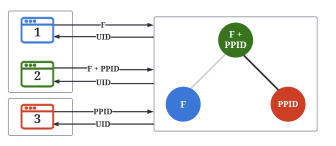
\includegraphics[scale=0.5]{img/crosssite}
\end{figure}

\begin{enumerate}
\item User visits a website on the first device. ID is set.
\item User logs in on that device - a piece of personally identifiable information (PPID - \textit{Publisher-Provided ID}) is connected to that ID.
\item User logs in to another website. Gets another ID. Uses the same email to log in. Now those two IDs are connected.
\end{enumerate}

\end{frame}

\begin{frame}
\frametitle{How does 3rd Party Cookie Blocking impact tracking?}
\centering
\textit{Not much.}

\end{frame}

\begin{frame}
\frametitle{Impact of blocking 3rd party cookies}

\begin{itemize}
\item Blocking 3rd party cookies results in a negligible reduction of tracking requests.
\item Sites do not rely on third party cookies to track users.
\end{itemize}

\begin{figure}
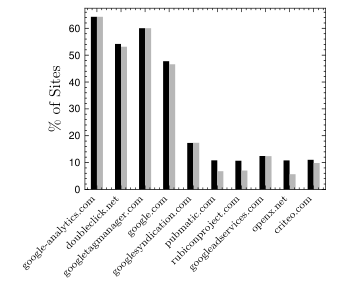
\includegraphics[scale=0.5]{img/trackingwhen3rdpcblock}
\end{figure}
\end{frame}



\section{Introducing CookieGraph}

\begin{frame}
\frametitle{CookieGraph}

\begin{figure}
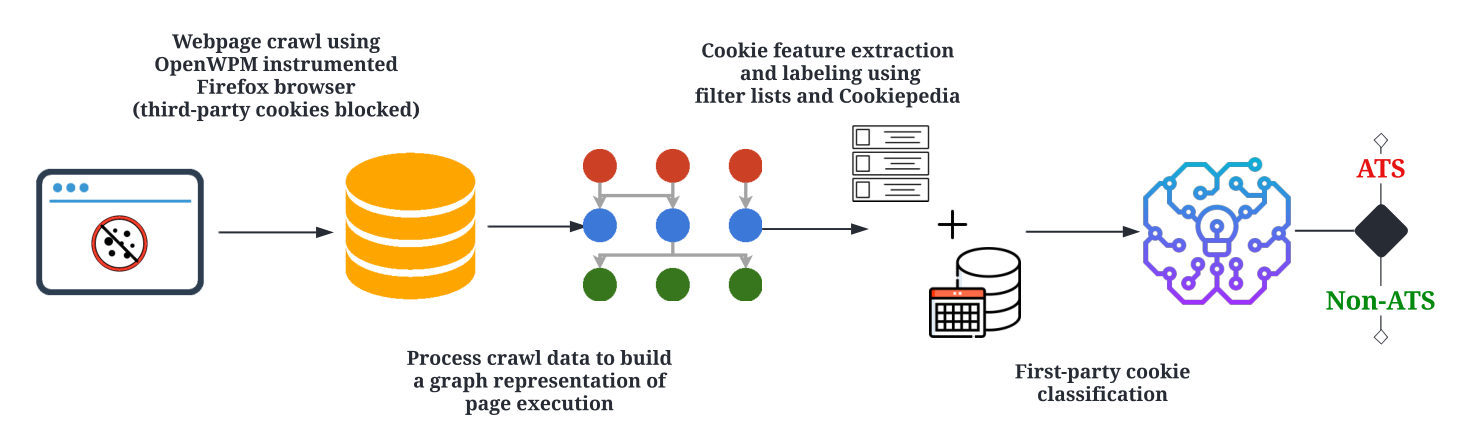
\includegraphics[scale=0.2]{img/diagram}
\end{figure}

\end{frame}

\begin{frame}
\frametitle{Design}

\begin{figure}
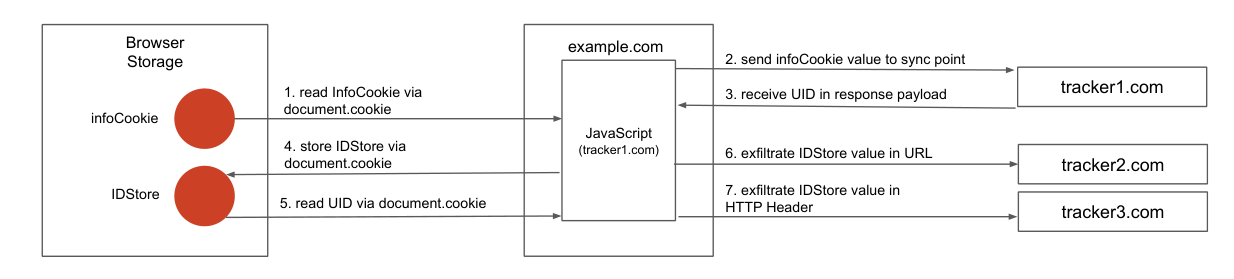
\includegraphics[scale=0.2]{img/graphconstruction}
\end{figure}

\begin{enumerate}
\item Crawl webpages
\item Build a graph representation of execution
\item Label data using other services like filter lists and Cookiepedia.
\item First-party cookie classification.
\end{enumerate}

\end{frame}

\begin{frame}
\frametitle{Crawl as much info as possible about a webpage}
\begin{itemize}
\item HTML elements
\item scripts
\item network responses
\item identifiers from network requests/responses
\item operations on browser's storage
\end{itemize}
\end{frame}

\begin{frame}
\frametitle{Graph}
\begin{itemize}
\item Make a node for each type of element crawled.
\item Connect them based on their interactions.
\item Track identifiers through these interactions.
\end{itemize}

\pic{grapcon2}

\end{frame}

\begin{frame}
\frametitle{Feature Extraction}
\begin{itemize}
\item Extract two kinds of features: \textit{structural} and \textit{flow}.
\item Structural - relationships between the nodes in the graph.
\item Flow - behavior of cookies, like "number of times a cookie was infiltrated/exfiltrated."
\end{itemize}
\end{frame}

\begin{frame}
\frametitle{Classification}
\begin{itemize}
\item Filter lists
\item Cookiepedia
\end{itemize}
\end{frame}



\section{Evaluation}

\begin{frame}
\frametitle{Feature Analysis}

\begin{figure}
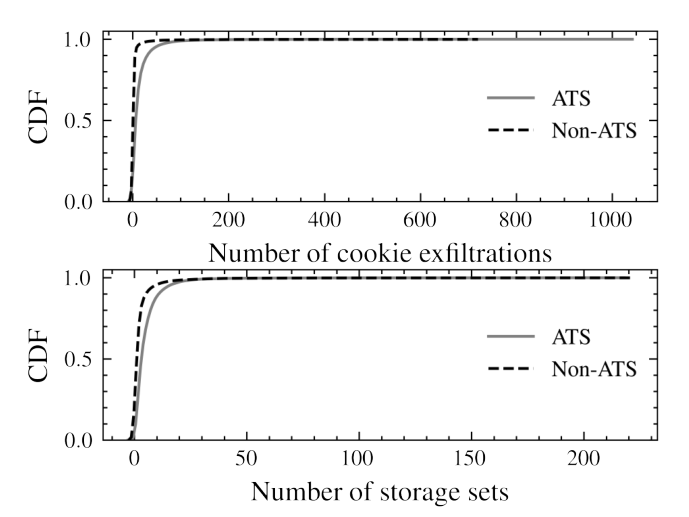
\includegraphics[scale=0.3]{img/featureanalysis}
\end{figure}

\end{frame}

\begin{frame}
\frametitle{Comparison with other technologies}

\begin{figure}
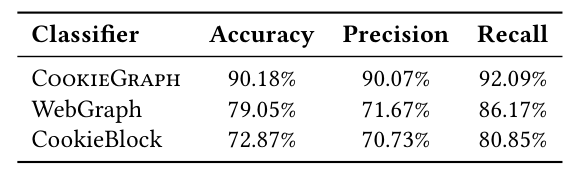
\includegraphics[scale=0.5]{img/classacc}
\end{figure}

\end{frame}

\begin{frame}
\frametitle{Measuring website breakage}

\begin{figure}
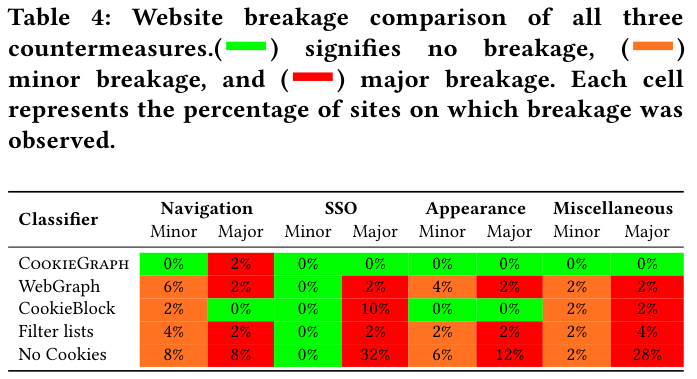
\includegraphics[scale=0.5]{img/breakage}
\end{figure}

\end{frame}

\begin{frame}
\frametitle{Prevalence of first-party tracking cookies}

\begin{itemize}
\item 89.86\% deploy at least one first-party tracking cookie.
\item Over 90\% are set by embedded third party scripts. 
\item Google and Facebook on at least one third of the sites.
\end{itemize}

\end{frame}

\begin{frame}
\frametitle{Limitiations}

\begin{itemize}
\item If there's not enough "website activity", some cookies are not detectable (eg. Criteo).
\item Large overhead prevents \textit{CookieGraph} from being run on user machines.
\end{itemize}

\end{frame}


\section{Summary}

\begin{frame}
\frametitle{Summary}

\begin{itemize}
\item Blocking third party cookies is ineffective in stopping tracking.
\item Almost 90\% of sites use tracking, first-party cookies.
\item \textit{CookieGraph} - detects tracking cookies based on site's behavior.
\item 90\% accuracy in detecting 1st party cookies, but cannot be run offline.
\end{itemize}

\end{frame}

\end{document}